

Sleep is an essential component of human health, contributing significantly to cognitive function, memory consolidation, and emotional regulation. Adequate and quality sleep ensures optimal brain performance and supports overall physical and mental well-being. Disruptions in sleep patterns can lead to various health issues, including impaired concentration, mood disorders, and chronic conditions such as cardiovascular diseases.

The classification of sleep stages is fundamental in understanding sleep architecture and diagnosing sleep disorders. Experts categorize sleep into five primary stages—N1, N2, N3, REM, and Wake—based on distinct patterns observed in brain activity. Each sleep stage is characterized by specific brainwave frequencies, which can be detected using electroencephalography (EEG) signals. Accurate classification of these stages is crucial for analyzing sleep quality and identifying abnormalities such as insomnia, sleep apnea, and narcolepsy.


Table~\ref{tab:sleep_stages} provides an overview of the frequency ranges associated with each sleep stage. 

\begin{table}[h]
\centering
\caption{Frequency ranges of different sleep stages.}
\begin{tabular}{ll}
\toprule
\textbf{Sleep Stage} & \textbf{Frequency Range (Hz)} \\
\midrule
Wake (Beta waves)       & 12--30 \\
N1 (Light Sleep)        & 4--8  \\
N2 (Moderate Sleep)     & 4--6  \\
N3 (Deep Sleep, Delta)  & 0.5--4  \\
REM (Theta waves)       & 4--6  \\
\bottomrule
\end{tabular}
\label{tab:sleep_stages}
\end{table}

To classify sleep stages effectively, bio-signals from multiple physiological channels are analyzed. The primary sources of information for sleep stage classification are EEG (electroencephalogram), EMG (electromyogram), and EOG (electrooculogram) signals. These channels capture brain activity, muscle movement, and eye movemets, respectively, offering a comprehensive view of sleep patterns.

\begin{figure}[!h]
    \centering
    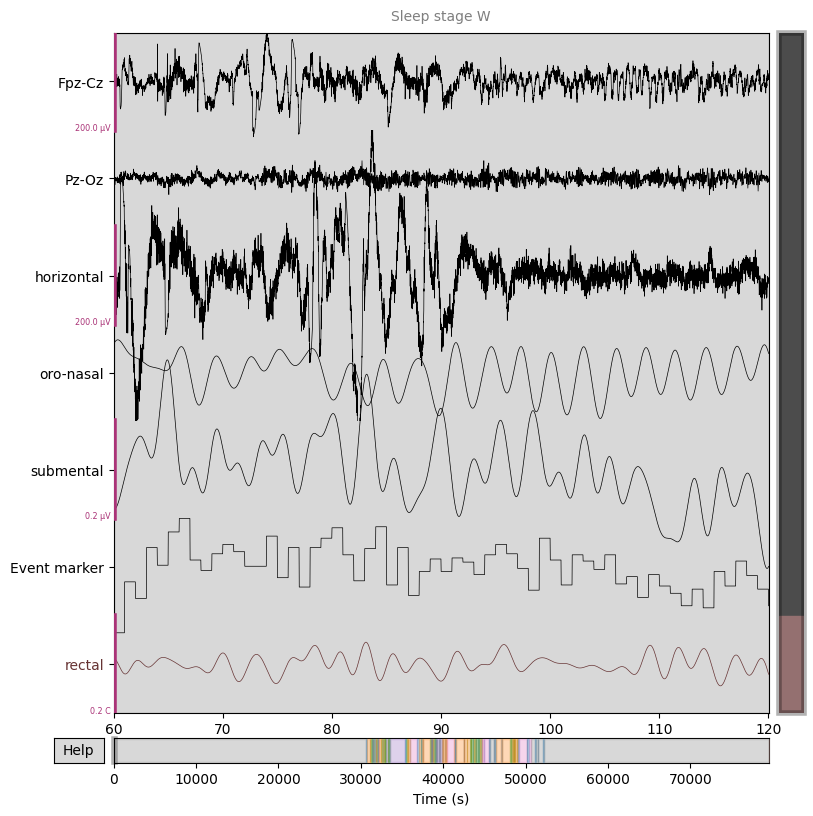
\includegraphics[width=0.5\linewidth]{img/Sleep EDF Data Visulization.png}
    \caption{Sleep EDF Data Visulization}
    \label{fig:enter-label}
\end{figure}

Despite the availability of multiple channels in the SleepEDF dataset, not all contribute equally to classification performance. To reduce model complexity without compromising accuracy, we selectively utilize four channels from the nine standard channels provided in the dataset. The selected channels are:

\begin{itemize}
    \item \textbf{EEG Fpz-Cz}: Captures frontal-to-central brain activity.  
    \item \textbf{EEG Pz-Oz}: Measures parietal-to-occipital brain activity.  
    \item \textbf{EMG submental}: Records muscle tone from the chin area.  
    \item \textbf{EOG horizontal}: Tracks horizontal eye movements.  
\end{itemize}

In this study, we adopt a graph-based modeling approach to capture spatial relationships between the selected channels. Additionally, we employ a Transformer encoder to effectively model temporal dependencies across sleep cycles. To facilitate a better understanding of the input data, we also present visualizations of bio-signals from all channels.

This approach aims to leverage the strengths of both spatial and temporal modeling techniques, resulting in a robust and efficient sleep stage classification framework.
